% Name: Rocket
% Description: A rocket with a red nose cone, a round window, two fins, and a flame from its nozzle.
% Tags: rocket, space, launch, illustration

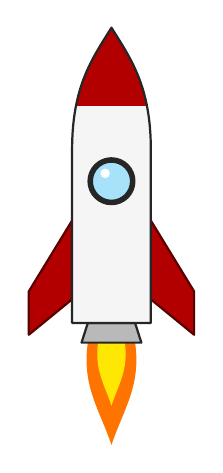
\begin{tikzpicture}[line join=round, thick]
  % Flame, behind everything
  \fill[orange!90!red] (-0.3,-0.25) .. controls (-0.38,-0.8) and (-0.15,-1.1) .. (0,-1.55) .. controls (0.15,-1.1) and (0.38,-0.8) .. (0.3,-0.25) -- cycle;
  \fill[yellow!90!orange] (-0.17,-0.25) .. controls (-0.22,-0.6) and (-0.08,-0.8) .. (0,-1.05) .. controls (0.08,-0.8) and (0.22,-0.6) .. (0.17,-0.25) -- cycle;
  % Nozzle
  \filldraw[fill=gray!55, draw=gray!30!black] (-0.3,0) -- (0.3,0) -- (0.38,-0.25) -- (-0.38,-0.25) -- cycle;
  % Fins
  \foreach \s in {-1,1}
    \filldraw[fill=red!70!black, draw=red!35!black] (0.5*\s,1.3) -- (1.05*\s,0.4) -- (1.05*\s,-0.15) -- (0.5*\s,0.3) -- cycle;
  % Body, with the nose cone painted inside a clip of it
  \path[save path=\body] (-0.5,0) -- (-0.5,2.2) .. controls (-0.5,3) and (-0.25,3.35) .. (0,3.75) .. controls (0.25,3.35) and (0.5,3) .. (0.5,2.2) -- (0.5,0) -- cycle;
  \fill[gray!8, use path=\body];
  \begin{scope}
    \clip[use path=\body];
    \fill[red!70!black] (-1,2.75) rectangle (1,4);
  \end{scope}
  \draw[gray!30!black, use path=\body];
  % Window
  \filldraw[fill=cyan!35, draw=gray!30!black, line width=2pt] (0,1.8) circle (0.27);
  \fill[white] (-0.08,1.9) circle (0.06);
\end{tikzpicture}
